
% =====================================================================
%  A0 landscape poster -- restructured three-column storyline
%  Machine Learning for 3D Geometry (SS 2026), TUM
%
%  Compile from this directory:
%      pdflatex poster_restructured.tex
%
%  Missing figures are replaced automatically by labelled placeholders.
% =====================================================================
\documentclass[a0,landscape]{a0poster}

\usepackage[utf8]{inputenc}
\usepackage[T1]{fontenc}
\usepackage{helvet}
\renewcommand{\familydefault}{\sfdefault}
\usepackage{sansmath}
\sansmath

\usepackage{graphicx}
\usepackage{booktabs}
\usepackage{array}
\usepackage{colortbl}
\usepackage[most]{tcolorbox}
\usepackage{tikz}
\usetikzlibrary{arrows.meta, positioning, calc, fit}
\usepackage{enumitem}
\usepackage{geometry}
\geometry{a0paper,landscape,margin=1.55cm}

\pagestyle{empty}
\parindent0pt

% ------------------------------- colors ------------------------------
\definecolor{tumblue}{HTML}{0065BD}
\definecolor{tumdark}{HTML}{003359}
\definecolor{tumlight}{HTML}{64A0C8}
\definecolor{tumpale}{HTML}{E8F0F7}
% Keep the visual language deliberately limited to the TUM blue family.
\definecolor{accent}{HTML}{0065BD}
\definecolor{accentpale}{HTML}{E8F0F7}
\definecolor{bodygrey}{HTML}{30343B}
\definecolor{cardgrey}{HTML}{F4F6F8}
\definecolor{success}{HTML}{238636}
\definecolor{lightgreen}{HTML}{E7F4EA}

\color{bodygrey}

% --------------------------- reusable boxes --------------------------
\newtcolorbox{posterbox}[2][]{%
  enhanced, breakable=false,
  colback=white, colframe=tumdark, boxrule=1.3pt, arc=4mm,
  left=8mm, right=8mm, top=12mm, bottom=6mm,
  before skip=8mm, after skip=0mm,
  attach boxed title to top center={yshift=-8mm},
  boxed title style={colback=tumdark, colframe=tumdark, arc=3mm,
                     left=13mm, right=13mm, top=3mm, bottom=3mm},
  title={\Large\bfseries\textcolor{white}{#2}}, #1}

\newtcolorbox{milestonebox}[3][]{%
  enhanced, breakable=false,
  colback=tumpale!42!white, colframe=tumblue, boxrule=1.25pt, arc=4mm,
  left=8mm, right=8mm, top=6mm, bottom=6mm,
  before skip=6mm, after skip=0mm,
  title={#2}, colbacktitle=tumblue, coltitle=white,
  fonttitle=\Large\bfseries, halign title=center,
  toptitle=3mm, bottomtitle=3mm, #1}

\newcommand{\pill}[2]{\tikz[baseline=-2mm]{\node[
  fill=#1, text=white, font=\large\bfseries, rounded corners=2.5mm,
  inner xsep=5mm, inner ysep=2.1mm]{#2};}}

% Use the real image when present; otherwise draw a labelled placeholder.
% Arguments: file, width, height, placeholder label.
\newcommand{\safeimage}[4]{%
  \IfFileExists{#1}{%
    \includegraphics[width=#2,height=#3,keepaspectratio]{#1}%
  }{%
    \begin{tikzpicture}
      \node[draw=tumlight, dashed, line width=1.2pt, rounded corners=3mm,
            fill=tumpale!45, minimum width=#2, minimum height=#3,
            text width=\dimexpr#2-14mm\relax, align=center,
            font=\normalsize\bfseries, text=tumdark]
            {FIGURE PLACEHOLDER\\[2mm]\normalfont #4};
    \end{tikzpicture}%
  }}

% Same fallback behaviour as \safeimage, but forces an exact image size.
% Useful for visually matching images with slightly different aspect ratios.
\newcommand{\safeimagefixed}[4]{%
  \IfFileExists{#1}{%
    \includegraphics[width=#2,height=#3]{#1}%
  }{%
    \begin{tikzpicture}
      \node[draw=tumlight, dashed, line width=1.2pt, rounded corners=3mm,
            fill=tumpale!45, minimum width=#2, minimum height=#3,
            text width=\dimexpr#2-14mm\relax, align=center,
            font=\normalsize\bfseries, text=tumdark]
            {FIGURE PLACEHOLDER\\[2mm]\normalfont #4};
    \end{tikzpicture}%
  }}

% Preserve the original aspect ratio while enforcing a shared visual height.
% This is used for side-by-side figures whose top and bottom edges must align.
\newcommand{\safeimageheight}[4]{%
  \IfFileExists{#1}{%
    \includegraphics[height=#3]{#1}%
  }{%
    \begin{tikzpicture}
      \node[draw=tumlight, dashed, line width=1.2pt, rounded corners=3mm,
            fill=tumpale!45, minimum width=#2, minimum height=#3,
            text width=\dimexpr#2-14mm\relax, align=center,
            font=\normalsize\bfseries, text=tumdark]
            {FIGURE PLACEHOLDER\\[2mm]\normalfont #4};
    \end{tikzpicture}%
  }}

\tikzset{
  method/.style={rectangle, rounded corners=3mm, draw=#1, fill=#1!8!white,
                 line width=1.2pt, inner sep=5mm, text width=0.88\linewidth,
                 align=left},
  feature/.style={rectangle, rounded corners=2.5mm, fill=tumpale,
                  draw=tumlight, line width=1pt, minimum height=14mm,
                  align=center, inner xsep=4mm},
  model/.style={rectangle, rounded corners=3mm, fill=tumblue, text=white,
                font=\normalsize\bfseries, minimum height=17mm,
                align=center, inner xsep=5mm},
  frozen/.style={rectangle, rounded corners=2.5mm, fill=cardgrey,
                 draw=bodygrey!45, minimum height=15mm, align=center,
                 inner xsep=4mm},
  trainable/.style={rectangle, rounded corners=2.5mm, fill=accentpale,
                    draw=accent, line width=1.3pt, minimum height=15mm,
                    align=center, inner xsep=4mm},
  arrow/.style={-{Latex[length=5mm]}, line width=1.5mm, draw=tumdark},
  thinarr/.style={-{Latex[length=3.5mm]}, line width=1mm, draw=tumdark},
}

\begin{document}

% =============================== HEADER ==============================
\begin{tcolorbox}[enhanced,colback=tumdark,colframe=tumdark,arc=6mm,
                  left=13mm,right=13mm,top=6mm,bottom=6mm]
  \begin{minipage}[c][52mm][c]{0.10\linewidth}
    \centering
    \safeimage{figures/qr.png}{34mm}{34mm}{QR code to repository}
  \end{minipage}\hfill
  \begin{minipage}[c][52mm][c]{0.78\linewidth}
    \centering
    \resizebox{0.98\linewidth}{!}{\textbf{\textcolor{white}{%
      Can a Vision--Language Model Improve the Grouping of 2D Masks into 3D Object Instances?}}}\\[7mm]
    {\LARGE\textcolor{tumlight}{\textbf{Samet Degirmenci
      \;\textperiodcentered\; Florian Wissel
      \;\textperiodcentered\; Katerina Skotnicova
      \;\textperiodcentered\; Omar Faheem}}}
  \end{minipage}\hfill
  \begin{minipage}[c][52mm][t]{0.10\linewidth}
    \raggedleft
    \vspace{0pt}
    {\fontsize{38}{40}\selectfont\bfseries\textcolor{white}{TUM}}
  \end{minipage}
\end{tcolorbox}

\vspace{1mm}
\noindent
% =====================================================================
% COLUMN 1 -- MOTIVATION + THREE METHODS (27%)
% =====================================================================
\begin{minipage}[t]{0.265\linewidth}
\vspace{0pt}

\begin{posterbox}[before skip=0mm]{Motivation}
  \begin{center}
    \safeimage{figures/masks_frame80.png}{0.72\linewidth}{88mm}%
      {Replica RGB frame with CropFormer masks}
  \end{center}
  \vspace{2mm}
  {\large Geometry groups \textbf{2D masks} consistently across views, but lacks
  the \textbf{semantic understanding} needed to resolve ambiguous object
  associations.}\\[4mm]
  \begin{tcolorbox}[colback=tumpale,colframe=tumlight,boxrule=1pt,arc=3mm,
                    left=5mm,right=5mm,top=3mm,bottom=3mm]
    \large\bfseries\textcolor{tumdark}{Research question:}\quad
    Can semantic evidence improve geometric mask grouping without requiring
    pairwise VLM inference?
  \end{tcolorbox}
\end{posterbox}

\begin{posterbox}[height=480mm]{Three Approaches We Compare}
  \pill{tumlight}{1 \; MaskClustering}\\[3mm]
  \begin{tcolorbox}[colback=tumpale!55,colframe=tumlight,boxrule=1pt,arc=3mm,
                    left=5mm,right=5mm,top=4mm,bottom=4mm]
    {\large\textbf{Geometric baseline}}\\[1mm]
    \normalsize View consensus $\rightarrow$ graph clustering
    $\rightarrow$ 3D instances. Efficient, but limited by geometric evidence.
  \end{tcolorbox}

  \vspace{4mm}
  \pill{tumblue}{2 \; Fine-tuned Qwen3-VL}\\[3mm]
  \begin{tcolorbox}[colback=tumblue!6,colframe=tumblue,boxrule=1pt,arc=3mm,
                    left=5mm,right=5mm,top=4mm,bottom=4mm]
    {\large\textbf{Semantic edge scorer}}\\[1mm]
    \normalsize Two outlined mask views $\rightarrow P(\text{same instance})$
    $\rightarrow$ graph clustering.
  \end{tcolorbox}

  \vspace{4mm}
  \pill{accent}{3 \; Fusion MLP (ours)}\\[3mm]
  \begin{tcolorbox}[colback=accentpale,colframe=accent,boxrule=1.2pt,arc=3mm,
                    left=5mm,right=5mm,top=4mm,bottom=4mm]
    {\large\textbf{Semantic--geometric fusion}}\\[1mm]
    \normalsize Qwen probability + geometric evidence $\rightarrow$ learned
    edge probability $\rightarrow$ graph clustering.
  \end{tcolorbox}

  \vspace{5mm}
  \begin{center}
    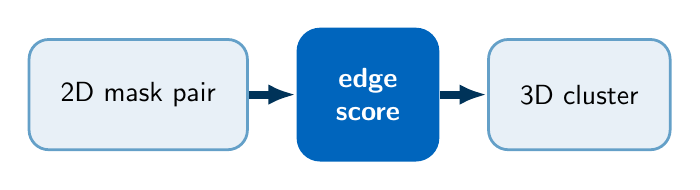
\begin{tikzpicture}[node distance=5mm]
      \node[feature] (m) {2D mask pair};
      \node[model,right=6mm of m] (s) {edge\\score};
      \node[feature,right=6mm of s] (c) {3D cluster};
      \draw[thinarr] (m)--(s);
      \draw[thinarr] (s)--(c);
    \end{tikzpicture}
  \end{center}
  {\normalsize\itshape The input masks and downstream clustering task are
  shared; the source of the edge evidence changes.}
\end{posterbox}

\end{minipage}\hfill
% =====================================================================
% COLUMN 2 -- FOUR MILESTONES (43%)
% =====================================================================
\begin{minipage}[t]{0.425\linewidth}
\vspace{0pt}

\begin{milestonebox}[before skip=0mm,top=4mm,bottom=4mm]{Milestone 1 \;\textperiodcentered\; Reproducing MaskClustering}{tumblue}
  \begin{minipage}[c]{0.42\linewidth}
    \raggedright
    \begin{tabular}{@{}c@{\hspace{2mm}}c@{}}
      \safeimage{figures/10.jpg}{0.48\linewidth}{52mm}{Replica frame 10} &
      \safeimage{figures/80.jpg}{0.48\linewidth}{52mm}{Replica frame 80}\\[2mm]
      \safeimage{figures/111.jpg}{0.48\linewidth}{52mm}{Replica frame 111} &
      \safeimage{figures/163.jpg}{0.48\linewidth}{52mm}{Replica frame 163}
    \end{tabular}
  \end{minipage}\hspace*{-5mm}
  \begin{minipage}[c]{0.28\linewidth}
    \centering
    \safeimageheight{figures/maskclustering_cluster_graph_cut.png}{0.98\linewidth}{106mm}%
      {MaskClustering instance graph 1}
  \end{minipage}\hfill
  \begin{minipage}[c]{0.28\linewidth}
    \centering
    \safeimageheight{figures/maskclustering_cluster_graph_2.png}{0.98\linewidth}{106mm}%
      {MaskClustering instance graph 2}
  \end{minipage}\hspace*{5mm}
\end{milestonebox}

\begin{milestonebox}{Milestone 2 \;\textperiodcentered\; Choosing the 2D Mask Generator}{tumblue}
  \begin{center}
    \begin{minipage}[t]{0.485\linewidth}
      \centering
      \begin{tabular}{@{}*{3}{>{\centering\arraybackslash}p{0.32\linewidth}}@{}}
        \large\bfseries\textcolor{tumdark}{CropFormer} &
        \large\bfseries\textcolor{tumdark}{SAM} &
        \large\bfseries\textcolor{tumdark}{SAM3}
      \end{tabular}\par\vspace{2mm}
      \safeimagefixed{figures/masks_1.png}{\linewidth}{86mm}%
        {CropFormer / SAM / SAM3 comparison 1}
    \end{minipage}\hfill
    \begin{minipage}[t]{0.485\linewidth}
      \centering
      \begin{tabular}{@{}*{3}{>{\centering\arraybackslash}p{0.32\linewidth}}@{}}
        \large\bfseries\textcolor{tumdark}{CropFormer} &
        \large\bfseries\textcolor{tumdark}{SAM} &
        \large\bfseries\textcolor{tumdark}{SAM3}
      \end{tabular}\par\vspace{2mm}
      \safeimagefixed{figures/masks_2.png}{\linewidth}{86mm}%
        {CropFormer / SAM / SAM3 comparison 2}
    \end{minipage}
  \end{center}
\end{milestonebox}

\begin{milestonebox}[height=160mm]{Milestone 3 \;\textperiodcentered\; Using Qwen3-VL and Fine-tuned Qwen3-VL}{tumblue}
  % \begin{center}
  %   \safeimage{figures/qwen_finetuning_architecture.png}{0.96\linewidth}{82mm}%
  %     {Qwen3-VL architecture with fine-tuned vision layers and MLP head}
  % \end{center}
    \begin{minipage}[t]{0.39\linewidth}
    {\large\bfseries\textcolor{accent}{High-recall candidate selection}}\\[1mm]
    {\normalsize Qwen inference on all $\mathcal{O}(N^2)$ pairs is too slow.
    We therefore retain a pair if \textbf{any} cheap criterion passes:}\\[-1mm]
    \begin{tcolorbox}[colback=white,colframe=accent,boxrule=1.1pt,arc=3mm,
                      left=5mm,right=5mm,top=2mm,bottom=4mm]
      \centering\large
      $\mathrm{DepthIoU}\geq\tau$\\[1mm]
      \textbf{OR} directional overlap $\geq\tau$\\[1mm]
      \textbf{OR} view consensus $\geq0.60$
    \end{tcolorbox}
    {\normalsize The relaxed OR rule aims to preserve positive pairs while
    reducing expensive VLM calls.}
  \end{minipage}\hfill
  \begin{minipage}[t]{0.58\linewidth}
    {\large\bfseries\textcolor{accent}{Fine-Tuned QWEN3-VL architecture}}\\[3mm]
    \centering
    \safeimage{figures/fusion_mlp_architecture.png}{0.96\linewidth}{108mm}%
      {QWEN3 Architecture and Fine-Tuned component}
  \end{minipage}

 
\end{milestonebox}

\begin{milestonebox}[height=265mm]
{Milestone 4 \;\textperiodcentered\; Efficient Semantic-Geometric Fusion}{tumblue}

% =====================================================================
% HORIZONTAL METHOD ROW
% =====================================================================

\noindent
% ---------------------------------------------------------------------
% 1. FEATURES
% ---------------------------------------------------------------------
\begin{minipage}[t]{0.24\linewidth}
\vspace{0pt}

{\large\bfseries\textcolor{accent}{1.\ Fusion features}}\\[2mm]

{\small
Each retained mask pair is represented by one semantic and five
geometric features.}

\vspace{2mm}

\begin{tcolorbox}[
  colback=tumpale!45!white,
  colframe=tumlight,
  boxrule=1pt,
  arc=3mm,
  left=4mm,
  right=4mm,
  top=3mm,
  bottom=3mm
]

\normalsize
\renewcommand{\arraystretch}{1.48}

\begin{tabular}{
@{}
>{\raggedright\arraybackslash}p{0.34\linewidth}
>{\centering\arraybackslash}p{0.56\linewidth}
@{}
}

\textcolor{tumblue}{\bfseries Semantic}
&
$p_{\mathrm{Qwen}}$
\\[1mm]

\textcolor{accent}{\bfseries Geometric}
&
$C_{\mathrm{view}}$
\\

&
$\log(1+N_{\mathrm{obs}})$
\\

&
$\mathrm{DepthIoU}$
\\

&
$O_{A\rightarrow B}$
\\

&
$O_{B\rightarrow A}$
\\

\end{tabular}

\end{tcolorbox}

\vspace{2mm}

% {\small
% $N_{\mathrm{obs}}$ is the number of observations supporting the pair.
% Both directional overlaps are retained because the relation is
% asymmetric.}

% \vspace{3mm}

% \begin{tcolorbox}[
%   colback=white,
%   colframe=tumlight,
%   boxrule=0.9pt,
%   arc=3mm,
%   left=4mm,
%   right=4mm,
%   top=2.5mm,
%   bottom=2.5mm
% ]
% \normalsize
% \textbf{Training target:}
% same-instance versus different-instance mask pairs from the Replica
% annotations.
% \end{tcolorbox}

\end{minipage}%
\hfill%
% ---------------------------------------------------------------------
% 2. MLP ARCHITECTURE
% ---------------------------------------------------------------------
\begin{minipage}[t]{0.40\linewidth}
\vspace{0pt}

{\large\bfseries\textcolor{accent}{2.\ Fusion MLP edge scorer}}\\[2mm]

\begin{center}
  \safeimage{figures/fusion_mlp/MLP_architecture.png}
    {0.98\linewidth}{105mm}
    {Six-input Fusion MLP architecture}
\end{center}


% \begin{tcolorbox}[
%   colback=accentpale,
%   colframe=accent,
%   boxrule=1.05pt,
%   arc=3mm,
%   left=4mm,
%   right=4mm,
%   top=3mm,
%   bottom=3mm
% ]
% \small

% For candidate pair $(u,v)$,

% \[
% \hat p_{uv}
% =
% P_{\mathrm{MLP}}
% \left(
% y_{uv}=1
% \mid
% \mathbf{x}_{uv}
% \right),
% \]
% with \[
% \mathbf{x}_{uv}
% =
% {[\$FEATURES]}
% \]

% \end{tcolorbox}



\end{minipage}%
\hfill%
% ---------------------------------------------------------------------
% 3. GRAPH CONSTRUCTION AND CLUSTERING
% ---------------------------------------------------------------------
\begin{minipage}[t]{0.34\linewidth}
\vspace{0pt}

{\large\bfseries\textcolor{accent}{3.\ MaskClustering integration}}\\[2mm]

\begin{center}
  \safeimage{figures/fusion_mlp/cluster_fusionMLP.jpeg}
    {0.95\linewidth}{105mm}
    {Fusion-score graph construction and clustering}
\end{center}


\end{minipage}

% =====================================================================
% REPLICA DATA SPLIT
% =====================================================================

\vspace{-10mm}

\begin{center}

{\large\bfseries\textcolor{tumdark}{Replica data split}}\\[2mm]

\renewcommand{\arraystretch}{1.0}

\begin{tabular}{@{}*{8}{c@{\hspace{2mm}}}@{}}

  \multicolumn{5}{c}{\textbf{Training}} &
  \textbf{\textcolor{tumblue}{Validation}} &
  \multicolumn{2}{c}{\textbf{\textcolor{tumdark}{Testing}}}
  \\[1.5mm]

  \safeimage{figures/room0.jpg}
    {0.108\linewidth}{38mm}{room0}
  &
  \safeimage{figures/office0.jpg}
    {0.108\linewidth}{38mm}{office0}
  &
  \safeimage{figures/office1.jpg}
    {0.108\linewidth}{38mm}{office1}
  &
  \safeimage{figures/office2.jpg}
    {0.108\linewidth}{38mm}{office2}
  &
  \safeimage{figures/room1.jpg}
    {0.108\linewidth}{38mm}{room1}
  &
  {
    \setlength{\fboxrule}{1.2mm}
    \setlength{\fboxsep}{0.8mm}
    \fcolorbox{tumblue}{white}{
      \safeimage{figures/office4.jpg}
        {0.098\linewidth}{34mm}{office4}
    }
  }
  &
  {
    \setlength{\fboxrule}{1.2mm}
    \setlength{\fboxsep}{0.8mm}
    \fcolorbox{tumdark}{white}{
      \safeimage{figures/room2.jpg}
        {0.098\linewidth}{34mm}{room2}
    }
  }
  &
  {
    \setlength{\fboxrule}{1.2mm}
    \setlength{\fboxsep}{0.8mm}
    \fcolorbox{tumdark}{white}{
      \safeimage{figures/office3.jpg}
        {0.098\linewidth}{34mm}{office3}
    }
  }
  \\[1.5mm]

  \small\textbf{room0}
  &
  \small\textbf{office0}
  &
  \small\textbf{office1}
  &
  \small\textbf{office2}
  &
  \small\textbf{room1}
  &
  \small\textbf{\textcolor{tumblue}{office4}}
  &
  \small\textbf{\textcolor{tumdark}{room2}}
  &
  \small\textbf{\textcolor{tumdark}{office3}}

\end{tabular}

\end{center}

\end{milestonebox}

\end{minipage}\hfill
% =====================================================================
% COLUMN 3 -- RESULTS + QUALITATIVE FIGURES + CONCLUSION (30%)
% =====================================================================
\begin{minipage}[t]{0.295\linewidth}
\vspace{0pt}

\begin{posterbox}[before skip=0mm]{Results \textperiodcentered\; Replica room2}
  \begin{center}
  \normalsize
  \renewcommand{\arraystretch}{1.15}
  \begin{tabular}{@{}>{\raggedright\arraybackslash}p{0.48\linewidth}rrr@{}}
    \toprule
    \textbf{Edge scorer} & \textbf{AP} & \textbf{AP@50} & \textbf{AP@25}\\
    \midrule
    View consensus (baseline) & 0.082 & 0.189 & 0.423\\
    Qwen zero-shot             & 0.019 & 0.032 & 0.105\\
    Qwen fine-tuned (LoRA)    & 0.018 & 0.033 & 0.173\\
    Average (Qwen + consensus)& 0.075 & 0.191 & 0.430\\
    \rowcolor{accentpale}
    \textbf{Fusion MLP (geo + Qwen)} & \textbf{0.083} & \textbf{0.205} & \textbf{0.441}\\
    \bottomrule
  \end{tabular}
  \end{center}
  \vspace{3mm}
  {\normalsize\itshape Leak-free test scene (Qwen fine-tuned on
  office0/office1/room0). The Fusion MLP slightly beats the geometric baseline;
  simple averaging matches it and Qwen-only stays near zero. All variants share
  the same clustering and CropFormer masks.}

  \vspace{5mm}
  \begin{center}
  \normalsize
  \renewcommand{\arraystretch}{1.15}
  \begin{tabular}{@{}>{\raggedright\arraybackslash}p{0.48\linewidth}rrr@{}}
    \toprule
    \textbf{Mask backbone (M2)} & \textbf{AP} & \textbf{AP@50} & \textbf{AP@25}\\
    \midrule
    \rowcolor{accentpale}
    \textbf{CropFormer} & \textbf{0.149} & \textbf{0.305} & \textbf{0.489}\\
    SAM3 (conf 0.25)    & 0.123 & 0.224 & 0.370\\
    SAM1 (ViT-H)        & 0.061 & 0.107 & 0.222\\
    \bottomrule
  \end{tabular}
  \end{center}
\end{posterbox}

\begin{posterbox}{Qualitative Results}
  \begin{center}
    \begin{tabular}{@{}c@{\hspace{6mm}}c@{}}
      \pill{tumlight}{MaskClustering} & \pill{tumblue}{Qwen zero-shot}\\[3mm]
      \safeimage{figures/baseline.png}{0.46\linewidth}{56mm}{3D MaskClustering result} &
      \safeimage{figures/qwen_zeroshot.png}{0.46\linewidth}{56mm}{3D Qwen zero-shot result}\\[3mm]
      \pill{tumblue}{Qwen fine-tuned} & \pill{accent}{Fusion MLP}\\[3mm]
      \safeimage{figures/finetuned.png}{0.46\linewidth}{56mm}{3D fine-tuned Qwen result} &
      \safeimage{figures/fused.png}{0.46\linewidth}{56mm}{3D Fusion-MLP result}
    \end{tabular}
  \end{center}
  \vspace{2mm}
  \begin{center}
    \begin{tabular}{@{}c@{\hspace{6mm}}c@{}}
      \pill{tumlight}{Baseline (zoom)} & \pill{accent}{Fusion MLP (zoom)}\\[2mm]
      \safeimage{figures/table_baseline.png}{0.46\linewidth}{44mm}{Zoom-in on dining table: baseline} &
      \safeimage{figures/table_fused.png}{0.46\linewidth}{44mm}{Zoom-in on dining table: fusion MLP}\\[2mm]
      \safeimage{figures/chair_baseline.png}{0.46\linewidth}{44mm}{Zoom-in on chair: baseline} &
      \safeimage{figures/chair_fused.png}{0.46\linewidth}{44mm}{Zoom-in on chair: fusion MLP}
    \end{tabular}
  \end{center}
  {\normalsize\itshape Top: full predicted 3D instances (one color = one
  instance). Bottom: zoom-ins on the \textcolor{red}{dining table} (top) and a
  \textcolor{red}{chair} (bottom); both baseline and Fusion MLP correctly group
  each into a single instance.}
\end{posterbox}

\begin{posterbox}{Takeaway \& Outlook}
  \begin{tcolorbox}[colback=accentpale,colframe=accent,boxrule=1.2pt,arc=3mm,
                    left=6mm,right=6mm,top=5mm,bottom=5mm]
    {\large\bfseries\textcolor{accent}{KEY TAKEAWAY}}\\[2mm]
    {\large On Replica, geometry carries most of the signal: learned fusion
    slightly beats the baseline, while the fine-tuned VLM alone collapses
    objects together. LoRA likely hurts due to too little training data.}
  \end{tcolorbox}
  \vspace{3mm}
  \begin{itemize}[leftmargin=10mm,itemsep=1.0mm,topsep=0.5mm]
    \item Measure candidate recall versus the number of Qwen calls.
    \item Optimize compute requirements when using VLMs with a better approach.
    \item Evaluate robustness using larger VLMs and more fine-tuning data.
  \end{itemize}
\end{posterbox}

\end{minipage}

% ------------------------------ FOOTER -------------------------------
\begin{tikzpicture}[remember picture,overlay]
  \node[anchor=south west,text=tumdark,font=\large\itshape] (foot)
    at ([xshift=18mm,yshift=2mm]current page.south west)
    {Machine Learning for 3D Geometry (SS 2026)
     \;\textbar\; Technical University of Munich};
  \node[anchor=south east,text=tumdark,font=\footnotesize,align=right]
    at ([xshift=-18mm,yshift=2mm]current page.south east)
    {\textbf{References:}\;
     [1] Yan et al., \textit{MaskClustering}, CVPR 2024.\;
     [2] Qin et al., \textit{Qwen3-VL}, 2025.\;
     [3] Qi et al., \textit{CropFormer}, ICCV 2023.\;
     [4] Kirillov et al., \textit{SAM}, ICCV 2023.};
\end{tikzpicture}

\end{document}
